\documentclass[output=paper]{langsci/langscibook} 
\author{Christopher Lucas\affiliation{SOAS University of London}\lastand 
 Stefano Manfredi\affiliation{CNRS, SeDyL}
}
\title{Introduction}
% \keywords{} 
\abstract{This introductory chapter gives an overview of the aims, scope, and approach of the volume, while also providing a thematic bibliography of the most significant previous literature on Arabic and contact-induced change.}
\maketitle

\begin{document}\label{introintro}

\section{Rationale}
With its lengthy written history, wide and well-studied dialectal variation, and involvement in numerous heterogeneous contact situations, the Arabic language has an enormous contribution to make to our understanding of how language contact can lead to change. Until now, however, most of what is known about the diverse outcomes of contacts between Arabic and other languages has remained inaccessible to non-specialists. There are brief summary sketches \citep{Thomason2011,Versteegh2001article,Versteegh2010,Manfredi2018}, as well as a recent collection of articles on a range of issues connected with Arabic and language contact in general \citep{ManfrediTosco2018}, but no larger synthesis of the kind that is available, for example, for Amazonian languages \citep{Aikhenvald2002}.

Arabic has thus played little part in work to date on contact-induced change that is crosslinguistic in
scope (though see \citealt{Matras2009,Trudgill2011} for partial exceptions). By providing the community of general and historical linguists with the present collaborative synthesis of expertise on Arabic and contact-induced change, we hope to help rectify this situation. The work consists of twenty-nine chapters by leading authorities in their fields, and is divided into three Parts: overviews of contact-induced change in individual Arabic varieties (Part I); overviews of the outcomes of contact with Arabic in other languages (Part II); and overviews of various types of changes across Arabic varieties, in which contact has played a significant role (Part III). Chapters in each of the three Parts follow the fixed broad outlines detailed below in §\ref{introstructure}, in order to maximize coherence and ease of reference. All authors have also been encouraged a) to ensure their chapters contain a rich set of (uniformly glossed and transcribed) linguistic data, including original data where appropriate, and b) to provide as much sociohistorical data as possible on the speech communities involved, framed where possible with reference to Van Coetsem’s (\citeyear{VanCoetsem1988,VanCoetsem2000}) distinction between changes due to borrowing (by agents dominant in the recipient language (RL)) and imposition (by agents dominant in the source language (SL); see §\ref{introvc} for further details). These features are aimed at ensuring that the data presented in the volume can be productively drawn upon by scholars and students of linguistics who are not specialists in
Arabic linguistics, and especially those working on the mechanisms, typology, outcomes, and theory of contact-induced change cross-linguistically. 

The rest of this introductory chapter is structured as follows. We begin by providing a thematic bibliography of existing work on Arabic and contact-induced change in §\ref{introexistingwork}. The overall scope of the present volume is then detailed in §\ref{introscope}: §\ref{introwherewhat} locates and classifies the different varieties of what is called ``Arabic'' according to Jastrow's (\citeyear{Jastrow2002}) three geographic zones and Labov's (\citeyear{Labov2007}) concepts of transmission and diffusion in language change; §§\ref{intropartIoverview}--\ref{intropartIIIoverview} provide an overview of the content of each of the three Parts into which the present volume is divided. In §\ref{introvc} we give details of Van Coetsem's (\citeyear{VanCoetsem1988,VanCoetsem2000}) model of contact-induced change, which contributors to the volume have been encouraged to have reference to in their classification of the changes they describe. Details of the common structure and transcription and glossing conventions of the volume are then given in §\ref{introstructure}, and this introductory chapter finishes with §\ref{introthemes}, in which we draw out some of the key themes and future directions that emerge from the volume.


\section{Previous work}\label{introexistingwork}

As noted in §\ref{introintro}, there is a reasonably large existing literature focusing on specific aspects of Arabic and contact-induced change. For reviews of much of this literature, readers are referred to the relevant chapters of the present volume. Here we simply present the key works for ease of reference in the following (non-comprehensive) thematic bibliography.

\newpage
\begin{itemize}[noitemsep,leftmargin=11pt]
\item[\adfhalfrightarrowhead]Old Arabic and Middle Aramaic: \citet{Fraenkel1886}, \citet{Stein2018}, \citet{Retsö2011}, \citet{Weninger2011Aramaic}.

\item[\adfhalfrightarrowhead]Arabic and Neo-Aramaic: \citet{Sabar1984},
\citet{ArnoldBehnstedt1993}, \citet{Khan2002}, \citet{Arnold2007}, \citet{Borg2008}, Coghill (\citeyear{Coghill2010,Coghill2012,Coghill2015}), \citet{Jastrow2015}, \citet{Owens2016Aramaic}.

\item[\adfhalfrightarrowhead]Arabic and Hebrew:
\citet{Blau1981}, \citet{Nevo1999}, \citet{Yoda2013}, \citet{Horesh2015}.

\item[\adfhalfrightarrowhead]Arabic and (Modern) South Arabian languages: \citet{Diem1979}, \citet{Lonnet2011}, \citet{Zammit2011}, \citet{Watson2018}.

\item[\adfhalfrightarrowhead]Arabic and Indo-Iranian languages: Asbaghi (\citeyear{Asbaghi1987,Asbaghi2011}), \citet{Tsabolov1994}, \citet{Ingham2005}, Matras (\citeyear{Matras2007Domari,Matras2012}), \citet{Gazsi2011}, \citet{Ṣādiqī2011}, \citet{WalAnonby2015}, \citet{Herin2018}.

\item[\adfhalfrightarrowhead]Arabic and Turkish: \citet{BenCheneb1922}, \citet{Reinkowski1995}, Procházka (\citeyear{Procházka2002Adana,Procházka2011Turkish}), \citet{Isaksson2005}, \citet{SánchezVicente2012}, \citet{Haig2014}, \citet{Taylan2017}, \citet{AkkusBenmamoun2018}, \citet{Procházka-Eisl2018}.

\item[\adfhalfrightarrowhead]Arabic and Berber: Corriente (\citeyear{Corriente1998Berber,Corriente2002}), Taine-Cheikh (\citeyear{Taine-Cheikh1997Zenaga,Taine-Cheikh2008chapter,Taine-Cheikh2012,Taine-Cheikh2018quadri}), \citet{Brahimi2000}, \citet{Ameur2008}, Kossmann
(\citeyear{Kossmann2009,Kossmann2010,Kossmann2013book,Kossmann2013chapter,Kossmann2014}), Souag (\citeyear{Souag2007,Souag2009,Souag2013book,Souag2018berber,Souag2018thing}), Lafkioui (\citeyear{Lafkioui2013reinventing,Lafkioui2013bu}), \citet{Tigziri2008}, \citet{ElAissati2011}, \citet{vanPuttenSouag2015}, \citet{vanPuttenBenkato2017}.

\item[\adfhalfrightarrowhead]Arabic and (sub-)Saharan languages: \citet{Owens2000article,Owens2015,Owens2016idioms}, \citet{OwensHassan2004}, \citet{Souag2013lexical,Souag2016sahara}.

\item[\adfhalfrightarrowhead]Arabic and Latin/Romance languages: \citet{Brunot1949}, \citet{Benoliel1977}, Corriente (\citeyear{Corriente1978,Corriente1992chapter,Corriente1992book,Corriente2000,Corriente2005,Corriente2008}), \citet{Talmoudi1986}, \citet{Abdu1988}, Heath (\citeyear{Heath1989,Heath1999,Heath2015}), \citet{Cifoletti1994}, Ferrando (\citeyear{Ferrando1995,Ferrando1997}), \citet{OuldMohamedBaba2003}, \citet{Vicente2006}, Sayahi
(\citeyear{Sayahi2011,Sayahi2014,Sayahi2015}), \citet{Danna2018phonetic}.

\item[\adfhalfrightarrowhead]Contact influences on Classical and Modern Standard Arabic: \citet{Jeffrey2007} [1938], \citet{Blau1969}, \citet{Hebbo1984}.

\item[\adfhalfrightarrowhead]Contact influence in Mesopotamian Arabic: Masliyah (\citeyear{Masliyah1996,Masliyah1997}), \citet{MatrasShabibi2007}, \citet{ElZarkaZiagos2019}.

\item[\adfhalfrightarrowhead]Contact influence in Central Asian Arabic: \citet{Jastrow2005}, \citet{Ratcliffe2005}, \citet{Ingham2011afg}.

\item[\adfhalfrightarrowhead]Contact influence in Levantine Arabic: \citet{Barbot1961}, Halasi-Kun (\citeyear{Halasi-Kun1969,Halasi-Kun1973,Halasi-Kun1982}), \citet{Hopkins1995}, \citet{Contini1999}, \citet{Neishtadt2015}.

\item[\adfhalfrightarrowhead]Contact influence in Cypriot Arabic: \citet{Newton1964}, \citet{Tsiapera1964}, Borg (\citeyear{Borg1985,Borg1997CMA,Borg2004}), \citet{Roth2004}, \citet{Gulle2016}.

\item[\adfhalfrightarrowhead]Contact influence in Maltese: \citet{colin1957}, \citet{Aquilina1958}, \citet{krier1976}, \citet{Drewes1994}, \citet{mifsudloanverbs}, \citet{stolz2003}, \citet{vella2003}, \citet{bovingdondalli2006}, Brincat (\citeyear{brincat1996,brincat2011}), \citet{comriespagnol2016},  \citet{Souag2018berber}.

\item[\adfhalfrightarrowhead]Arabic pidgins and creoles: \citet{Owens1985}, \citet{BurengVincent1986}, Miller (\citeyear{Miller1989,Miller1993}), \citet{Nakao2012}, \citet{Luffin2014}, \citet{Manfredi2014relex}, Avram (\citeyear{Avram2017article,Avram2019}), \citet{Bizri2018}, \citet{Owens2018}

\item[\adfhalfrightarrowhead]Contact between Arabic dialects: \citet{Behnstedt1994Dialektkontakt}, Al-Wer (\citeyear{Al-Wer2002furtherreading,Al-Wer2007,Al-Wer2014}), \citet{Gibson2002}, \citet{Miller2007}, \citet{Al-Essa2009}, \citet{Palva2009}, \citet{Vicente2010}, \citet{Alghamdi2014}, \citet{CotterHoresh2015}, \citet{Leddy-Cecere2018}.

\item[\adfhalfrightarrowhead]Differential object marking: \citet{Coghill2014}, \citet{dohla2016}, \citet{Souag2017clitic}.

\item[\adfhalfrightarrowhead]Negation: Lucas (\citeyear{Lucas2007,Lucas2012,Lucas2013}), \citet{Souag2009}, \citet{LucasLash2010}, \citet{BreitbarthWillisLucasinpress}.

\end{itemize}

\section{Scope}\label{introscope}

\subsection{Where and what is Arabic?}\label{introwherewhat}

Arabic is one of the most widely spoken languages in the world and the first language of around 350 million speakers spread throughout the Middle East and North Africa. There are twenty-five sovereign states in which Arabic is an official language. In addition, Arabic is widely spoken as a lingua franca (i.e. vehicular language) for a range of communicative interactions between different linguistic communities in Asia and Africa. Following Jastrow (\citeyear{Jastrow2002}; see also \citealt{Watson2011dialectsoverview}; \citealt{Manfrediforthcoming}), the present-day Arabic-speaking world can be broadly subdivided into three geographic zones (cf. Figure \ref{intromap}): Zone I covers the regions of the Arabian Peninsula where Arabic was spoken before the beginning of the Islamic expansion in the seventh century; Zone II embraces the Middle Eastern and North African areas into which Arabic penetrated during the Islamic expansion, and where it is nowadays spoken as a majority language; Zone III encompasses isolated regions where Arabic is spoken by minority bilingual communities (see also \citealt{Owens2000editor}). Further to this, following successive waves of mass emigration in recent centuries, Arabic is also spoken as a heritage language by diasporic communities around the world (\citealt{Rouchdy_arabic_1992,BoumansdeRuiter2002}; D’Anna, this volume).\ia{D'Anna, Luca@D'Anna, Luca}. Against the backdrop of this complex geo-historical distribution, the question that arises is what unites all the varieties that fall under the glottonym ``Arabic'' and, more generally, what should count as Arabic from a linguistic point of view?

\begin{figure}
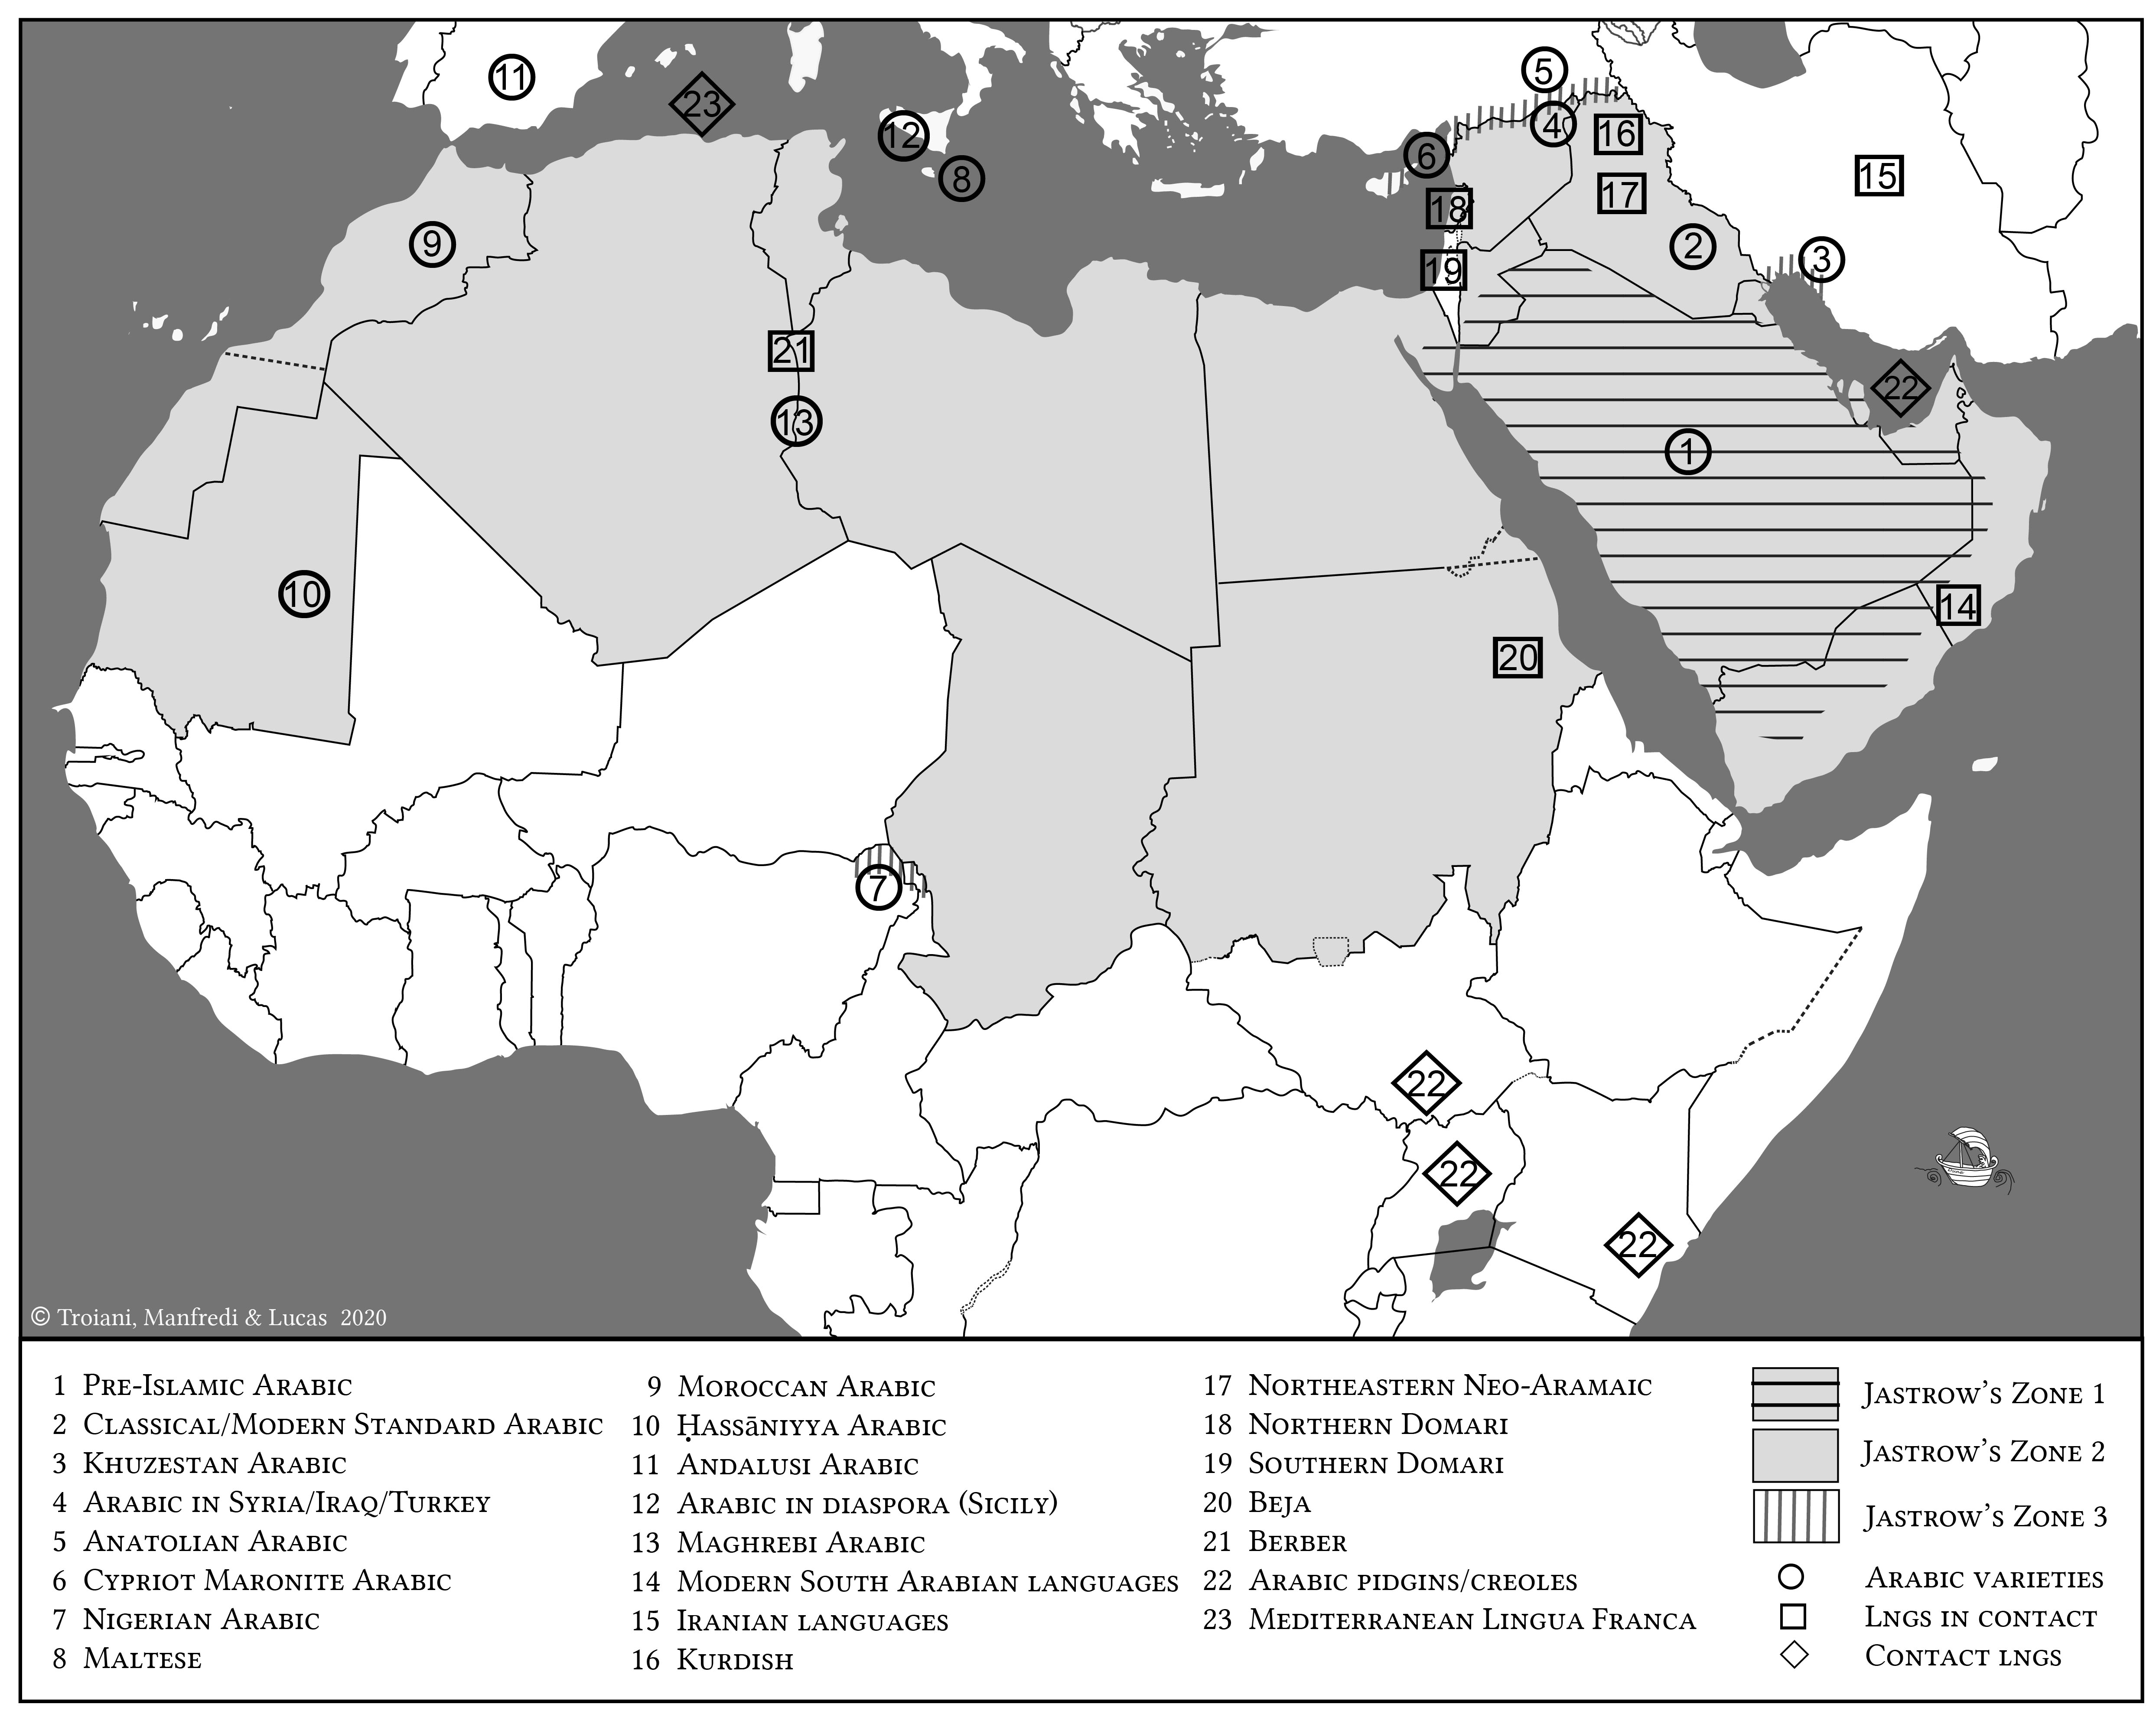
\includegraphics[width=\textwidth]{figures/intromap.jpg}
\caption{Approximate distruibution of languages and Arabic varieties discussed in this volume}
\label{intromap}
\end{figure}

After all, the term ``Arabic'' encompasses a great deal of internal variety, whose origins can be traced back to both internally and externally motivated (i.e. contact-induced) changes. \textcolor{red}{[I removed a sentence here as I didn't really understand it and it sounded subjective/unfalsifiable to me. We can always re-express it and put it back in.]}. One way of understanding these different patterns of language change is through Labov's (\citeyear{Labov2007}) distinction between \textsc{transmission} and \textsc{diffusion}. If transmission refers to change through an unbroken sequence of first language acquisition (\citealt{Labov2007}: 346), diffusion rather implies the transfer of features across languages via language/dialect contact (\citealt{Labov2007}: 347). Change through transmission is said to be regular because it is incremented by young native speakers, whereas diffusion is thought to be more irregular and unpredictable because it is typically produced by adult bilingual speakers. Both mechanisms contribute to long-term language change even though, according to Labov, transmission is the foremost mechanism by which linguistic diversity is produced and maintained. In a recent study, \citet{Owens2018} tests the generality of the Labovian distinction between transmission and diffusion against the complex linguistic and sociohistorical patchwork of Arabic. He concludes that change through diffusion cannot be said to be more irregular than change via transmission and that, other than for Arabic-based creoles (see Avram, this volume),\ia{Avram, Andrei@Avram, Andrei} there are no clear-cut criteria for distinguishing the two mechanisms of language change. The reason for this is that most of the linguistic varieties that are commonly referred to under the heading of ``Arabic'' are the result of a longstanding series of multi-causal changes encompassing both internal drift and convergence, as well as contact-induced change via diffusion. What we do not see, however, in any of the varieties usually referred to as Arabic are the atypical kinds of changes produced by the disruption of language transmission as observed in pidgin and creole languages (but see below). Accordingly, Part I of this volume primarily (but not exclusively) deals with contact-induced change in spoken varieties of Arabic that have gone through an unbroken chain of language transmission, the so-called ``Arabic dialects''. 

\subsection{Overview of Part I: Contact-induced change in varieties of Arabic}\label{intropartIoverview}

The survey chapters in Part I of this volume offer an extensive overview of contact-induced change in both Eastern (i.e. \textit{mašriqī}) and Western (i.e. \textit{maɣribī}) Arabic dialects (to use the terminology of the traditional geographical classification of modern Arabic dialects; cf. \citealt{Palva2009}; Benkato, this volume)\ia{Benkato, Adam@Benkato, Adam}. The majority of chapters in this Part describe varieties spoken by bilingual minorities affected to different degrees by language shift towards local dominant languages. For instance, the Arabic-speaking Maronite minority of Kormakiti is involved in an asymmetric pattern of bilingualism reulting in a gradual and inexorable language shift towards Cypriot Greek (Mary Ann Walter, this volume).\ia{Walter, Mary Ann@Walter, Mary Ann} In contrast, speakers of Nigerian Arabic (Jonathan Owens, this volume),\ia{Owens, Jonathan@Owens, Jonathan} despite considerable proficiency in Kanuri and/or Hausa, maintain transmission of their ancestral language to the younger generations. As far as it is possible to tell, a similar situation holds for the Mesopotamian dialects of Anatolia (Faruk Akkuş, this volume)\ia{Akkuş, Faruk@Akkuş, Faruk} and Khuzestan, (Bettina Leitner, this volume)\ia{Leitner, Bettina@Leitner, Bettina} which are in intense contact with Turkish and Persian respectively (among other languages), but without (yet) showing signs of definitive language shift. Procházka (this volume),\ia{Procházka, Stephan@Procházka, Stephan} on the other hand, describes the effects of contact-induced change in a continuum of Eastern Arabic dialects dispersed across Lebanon, Syria, Iraq, and southern Turkey. In this broader geographical context, Arabic represents the main vernacular language, affected to different degrees by long-term bi- or multilingualism with Aramaic, Kurdish, and Turkish.

As far as Western Arabic dialects are concerned, Benkato (this volume)\ia{Benkato, Adam@Benkato, Adam} describes a history of contact-induced change in different Maghrebi dialects from the beginning of the Arabization of North Africa until the colonial period. Four further chapters then take a closer look at contact-induced changes in specific varieties of Western Arabic. Heath (this volume)\ia{Heath, Jeffrey@Heath, Jeffrey} covers Moroccan, while Taine-Cheikh (this volume)\ia{Taine-Cheikh, Catherine@Taine-Cheikh, Catherine} covers Ḥassāniyya -- two majority varieties of Arabic historically affected by contact with Berber and Romance languages. Lucas \& Čéplö (this volume)\ia{Lucas, Christopher@Lucas, Christopher}\ia{Čéplö, Slavomír@Čéplö, Slavomír} then provide an overview of contact-induced change in Maltese -- a variety which is no longer usually considered to be a subtype of ``Arabic'', but which, as Lucas \& Čéplö (this volume) show, is nevertheless historically part of the Western group of Arabic dialects. Indeed, despite the far-reaching lexical and grammatical effects of contact with Italo-Romance and English, Maltese remains largely a product of transmission in the Labovian sense. We would not therefore classify it as a contact (i.e. mixed) language (cf. \citealt{stolz2003} and see further below). Lastly, D’Anna (this volume)\ia{D'Anna, Luca@D'Anna, Luca} offers a linguistic account of different varieties of Arabic in diasporic settings, with particular focus on the Tunisian community of Mazara del Vallo in Sicily. Unlike the Western varieties described in the aforementioned chapters, in this latter context Arabic is involved in an unbalanced contact situation, resulting in moderate language shift towards Sicilian and Italian.

As well as the aforementioned spoken varieties of Arabic, Part I of the volume also includes three chapters analysing the outputs of language contact in different varieties of written Arabic. First of all, Al-Jallad (this volume)ia{Al-Jallad, Ahmad@Al-Jallad, Ahmad} describes a number of likely instances of contact-induced change in pre-Islamic Arabic documentary sources (primarily inscriptional), and postulates the existence of different patterns of bilingualism between Arabic and Akkadian, Aramaic, Ancient South Arabian languages, and Greek (among other languages). Van Putten (this volume)\ia{van Putten, Marijn@van Putten, Marijn} then focuses on contact influences on the later Classical and Modern Standard Arabic, examining both early influences from Aramaic, Greek, Persian, Ethio-Semitic and Ancient South Arabian, as well as later influence from Ottoman Turkish and twentieth-century journalism in European languages. Since these written varieties of Arabic are rather artificial constructs, van Putten also examines the influence of the native Arabic dialects of the authors of texts in Classical and Modern Standard Arabic. The third and final written Arabic variety analysed in this volume is Andalusi Arabic. Attested as a form of Middle Arabic (\citealt{Lentin2011Middle}) between the tenth and seventeenth centuries, Andalusi Arabic displays significant grammatical and lexical input from both Romance and Berber languages (Vicente, this volume).\ia{Vicente, Ángeles@Vicente, Ángeles} As evidence for the Arabic varieties described in these three chapters is exclusively written, they cannot be treated in the same manner as spoken varieties which emerged in a context of first language acquisition. They are, however, representative of a longstanding and uninterrupted written tradition that goes back to the pre-Islamic period, and that has always been in a multi-faceted relationship of mutual influence with different varieties of spoken Arabic. In this sense, despite their rather artificial nature, written varieties of Arabic may also be considered the product of language transmission. 

In the final chapter of Part I, on the other hand, Avram (this volume)\ia{Avram, Andrei@Avram, Andrei}  describes a number of Arabic-based pidgins and creoles, which contrast with modern Arabic dialects (including Maltese) in that they have emerged in contact situations where the available language repertoires did not provide an effective tool for communication (\citealt{BakkerMatras2013intro}: 1). These contact languages are thus the product of partial or full interruption of language transmission, and for this reason they fall outside the range of what is usually considered Arabic (i.e. they are not straightforwardly classifiable as genetically related to Arabic; cf. \citealt{McMahon2013}). In such contexts, the effects of language diffusion via second language acquisition are obviously more evident. The varieties discussed by Avram include the so-called Sudanic pidgins and creoles (i.e. Juba Arabic, Ki-Nubi, and Turku), which emerged in Sudan in the nineteenth century and are today scattered across East Africa, as well as a number of contact languages that have recently emerged in the context of labour migration to the Middle East: Gulf Pidgin Arabic, Pidgin Madame, Romanian Pidgin Arabic, and Jordanian Pidgin Arabic. Despite their different sociohistorical and ethnolinguistic backgrounds, the contact languages included in this chapter share many formal features as a result of the strong impact of second language acquisition of Arabic in extreme contact situations.

In sum, Part I of the present volume aims at a comprehensive overview of contact-induced changes in both spoken and written varieties of Arabic, as well as in Arabic-based contact languages (but see §\ref{introlimitations}).

\subsection{Overview of Part II: Language change through contact
with Arabic}\label{intropartIIoverview}

Throughout its history, Arabic has not only been subject to contact influence from other languages, but has also itself induced profound changes in the languages with which it has come into contact (see \citealt{Versteegh2001article} for a general overview). The latter topic is the focus of the chapters included Part II of the present volume. Let us note in this regard that, thanks to its religious function as the language of Islam, the linguistic influence of (Classical) Arabic has of course travelled well beyond the traditional borders of the Arabic-speaking world, and has affected linguistic communities that have never acquired Arabic as a second language. Such is the case, for example, of Indonesian and Swahili, whose lexica are characterized by a high proportion of Arabic-derived loanwords. In the present volume we largely disregard this kind of influence, however, as our focus is rather on the effects of language contact in communities characterized by a relatively high degree of societal bilingualism in Arabic. These bilingual communities typically fall within Jastrow’s zone II (see §\ref{introwherewhat} and Figure \ref{intromap}), and are therefore affected to varying degrees by language shift towards Arabic. 

Accordingly, the first two chapters of Part II focus on the structural effects of language contact with Arabic in two Semitic languages of the Middle East. First of all, Bettega \& Gasparini (this volume)\ia{Bettega, Simone@Bettega, Simone}\ia{Gasparini, Fabio@Gasparini, Fabio} provide an overview of Arabic influence on the Modern Southern Arabian languages (i.e. Mehri, Hobyōt, Ḥarsūsi, Baṭḥari, Śḥerɛt/Jibbāli and Soqoṭri) of Oman and Yemen. These minority languages are used in an asymmetric pattern of bilingualism with Arabic and have been strongly affected by contact with the dominant language, both in their lexicon and grammar. A similar situation is described by Coghill (this volume)\ia{Coghill, Eleanor@Coghill, Eleanor} for North-Eastern Neo-Aramaic (NENA), a group of closely related languages whose speakers are scattered across Iraq, Turkey, Syria and Iran (as well as in several diasporic communities around the world). Unlike for the Modern South Arabian languages, however, Arabic has only recently become the dominant language in much of the region where NENA languages are spoken, with Kurdish being the primary historical contact language for NENA. Nevertheless, the intensity of this contact, despite its relatively short duration, has been sufficient to result in a degree of influence on the grammar and lexicon of NENA languages, as Cogill demonstrates. Being closely related to Arabic, NENA and Modern South Arabian languages are incidentally particularly relevant to the question of the role played by language contact (i.e. diffusion) as opposed to internal drift (i.e. transmission) in the reconstruction of the Semitic language family.

The next two chapters in Part II deal with languages that are also genetically related to Arabic, though much more distantly. First of all, Souag (this volume)\ia{Souag, Lameen@Souag, Lameen} surveys some of the most prominent examples of the influence of Arabic on the numerous Berber languages spoken across North Africa and the Sahara. Though many Berber-speaking communities are in the process of language shift, different communities present different patterns of bilingualism. Tuareg, for example, has been least affected by contact with spoken Arabic, whereas smaller varieties, such as that of Awjila in Libya are severly endangered, with language shift to Arabic being rather far advanced \citep{vanPuttenSouag2015}. Berber as a whole thus represents a particularly rich source of data for the typology of changes brought about by contact with Arabic (see also \citealt{Kossmann2013book}). Vanhove (this volume),\ia{Vanhove, Martine@Vanhove, Martine} on the other hand, describes the influence of Arabic on Beja, a Northern Cushitic language mainly spoken in eastern Sudan. Probably due to their constituting a large proportion of population in this region, and in spite of their high degree of bilingualism with Sudanese Arabic, Beja speakers continue robust transmission of their ancestral language to younger generations and are therefore not involved in a process of language shift. Against this background, Beja offers interesting hints for the analysis of the morphological effects of contact with Arabic, especially in relation to the transfer of roots and patterns (see also \citealt{Vanhove2012}). 

Part II of the volume also provides data for the analysis of contact-induced changes that occurred in languages with no genetic relation with Arabic. These are all Indo-Iranian languages, spoken in a large area stretching from Iran in the east to Israel in the west. Gazsi (this volume)\ia{Gazsi, Dénes@Gazsi, Dénes} offers a wide-ranging survey of the mostly lexical influence of Arabic on Iranian languages, with a particular focus on New Persian and modern Persian dialects spoken in Iran. Öpengin (this volume)\ia{Öpengin, Ergin@Öpengin, Ergin} then describes the effects of contact with Arabic in Northern and Central Kurdish languages spoken in Turkey, Syria and Iraq. Due to the longstanding bilingualism with Arabic since the early phases of the Islamic expansion, Kurdish has been profoundly affected in its phonology and lexicon by contact with both Mesopotamian dialects and Classical Arabic. Lastly, two further chapters assess the changes produced by contact with Arabic in different varieties of Domari, an Indic language spoken by itinerant linguistic minorities in the Middle East. Matras (this volume)\ia{Matras, Yaron@Matras, Yaron} analyses the Southern variety of Domari, spoken in Jerusalem, which is reported to be extremely endangered, while Herin (this volume)\ia{Herin, Bruno@Herin, Bruno} focuses on the Northern varieties of Domari, spoken in Syria, Lebanon, Jordan and Turkey, which exhibit different degrees of linguistic vitality. In this overall situation, Domari has been thoroughly affected in all lexical and grammatical domains by contact with Arabic, with dialects of Syria and Turkey showing a lower degree of linguistic interference, while more southerly dialects are on the verge of extinction due to language shift.  

In the final chapter of Part II, Nolan (this volume)\ia{Nolan, Joanna@Nolan, Joanna} discusses another contact language with significant input from Arabic: Mediterranean Lingua Franca, a vehicular language spoken from the sixteenth to nineteenth centuries on the North African Barbary coast as an interethnic means of communication between various populations, including pirates and captured slaves. The lexicon and grammar Mediterranean Lingua Franca were apparently drawn from a wide range of Italo-Romance, Spanish, Portuguese, Franco-Provençal, Turkish, Greek and Arabic varieties. Although the fact that the contribution of Arabic to this language was relatively slight, a substantial proportion of its speakers had Arabic as their first language and inevitably therefore transferred Arabic features into this contact language.

\subsection{Overview of Part III: Domains of contact-induced
change across Arabic varieties}\label{intropartIIIoverview}
...

\subsection{Limitations}\label{introlimitations}

Inevitably with a project of this scale, it has not been possible to cover every  aspect of the topic that we would have liked to, and the chapters included necessarily represent a compromise between several different academic and practical considerations. Thus, while we have aimed for blanket coverage of languages and varieties of Arabic that have been significantly affected by contact, a number of omissions should be noted. 

\textcolor{red}{[Moved from Part I overview]} For example, Central Asian Arabic (see \citealt{Seeger2013article}), a minority variety of Arabic strongly affected by contact with Tajik and Uzbek, though it is cited a number of times for comparative purposes by several contributors, is not thoroughly analysed in a dedicated chapter. Similarly, the influence of Modern Hebrew on Palestinian Arabic in Israel (see \citealt{Horesh2015}) is not analysed in detail in this volume. Furthermore, apart from Nigerian Arabic, little is said about other vernacular and vehicular varieties of Arabic spoken in sub-Saharan Africa (see \citealt{Lafkioui2013book}).

\textcolor{red}{[Moved from Part II overview]} Similarly, the languages discussed in Part II are certainly not the only ones to have been affected by direct contact with Arabic. For instance, several Nilo-Saharan languages found in central and eastern Africa have historically been in contact with different varieties of Arabic. This is the case of Nubian, an Eastern Sudanic language spoken on the Egypt--Sudan border \citep{Rouchdy1980}. The same applies to a number of Niger-Kordofanian languages spoken in the Nuba Mountains region of Sudan, and among which we can mention the case of Koalib \citep{Quint2018}. As far as the Middle East is concerned, the influence of Arabic on the Armenian varieties spoken in Lebanon unfortunately remains unstudied, and the same is true for the Turkmen dialects of Iraq and Syria. \textcolor{red}{[Is anything maybe missing from Part III that we want to talk about here? Maybe differential object marking/clitic doubling? Anything else?]} 

Despite these descriptive gaps, the twenty-nine chapters included in this volume collectively have the merit of discussing a wide range of contact situations involving Arabic (balanced bilingualism, unbalanced bilingualism, pidginization and creolization), which cover a broad geographical area and lengthy timespan, thus giving a close-to-comprehensive picture of the currently known facts of Arabic and contact-induced change.

\section{Framework}\label{introvc}
The majority of works cited in §\ref{introexistingwork} (like the majority of work generally on contact-induced changes in specific languages) describe a set of linguistic outcomes of language contact, without addressing the cognitive and acquisitional processes that lead speakers to introduce and adopt changes of this kind. In the present volume, we have encouraged authors wherever possible to go beyond mere itemization of contact-induced changes, and to give consideration to the processes which are likely to have brought them about. Specifically, we have asked authors to analyse changes wherever possible in terms of the framework (and terminology) developed by Frans Van Coetsem (\citeyear{VanCoetsem1988,VanCoetsem2000}).

While there are various models of contact-induced change available (see e.g. \citealt{ThomasonKaufman1988,Johanson2002,Matras2009}), Van Coetsem's is preferable for our purposes, in that it allows us to distinguish the major types of contact-induced change, based on the cognitive statuses of the source and recipient languages in the minds of the bilingual speakers who are the agents of the changes in question. This model, which has gained greater prominence following Winford's (\citeyear{Winford2005,Winford2007,Winford2010}) work to popularize it (see also \citealt{Ross2013} for a broadly similar approach), makes a fundamental distinction between \textsc{borrowing} and \textsc{imposition} as the two major types of \textsc{transfer} (i.e. contact-induced change that has the effect of making the RL more closely resemble the SL in some respect).\footnote{Note that not all contact-induced changes involve transfer in this sense. See §\ref{introproblem} for details.} The distinction between borrowing and imposition boils down to whether the agents of a particular change (i.e. the bilingual speakers who first introduce it) are cognitively (not sociolinguistically) dominant in the SL or the RL. Lucas (\citeyear{Lucas2012,Lucas2015}) argues that this notion of dominance (which Van Coetsem himself does not define precisely) can be reduced to nativeness, and is thus not equivalent to temporary accessibility: borrowing (also referred to as change under RL agentivity) is when a speaker for whom the RL is a native language introduces changes to the RL based on an SL model; imposition (also referred to as change under SL agentivity) is when changes of this sort are made by a speaker for whom the SL is a native language. Imposition occurs essentially because adults, with their impoverished language acquisition abilities relative to young children, consciously or unconsciously draw on the resources of their native language to fill the gaps in their knowledge of the second language. Borrowing, on the other hand, occurs either as a deliberate enrichment of the native language with material drawn from the second language, or otherwise as a result of the ``inherent cognitive tendency to minimize the processing effort associated with the use of two (or more) languages'' (\citealt{Lucas2012}: 291). Imposition thus prototypically transfers more abstract structural features (e.g., for German native speakers speaking second-language English, syllable-final devoicing and lack of preposition stranding), whereas borrowing is prototypically associated with transfer of lexical and constructional material. 

This approach neatly complements Labov's distinction between transmission and diffusion. Labov (\citeyear{Labov2007}: 349) points out that ``transmission is the product of the acquisition of language by young children'' whereas ``most language contact is largely between and among adults'' and that the fundamental differences between child first language and adult second language acquisition (cf. \citealt{BleyVroman1989,BleyVroman2009,Meisel2011}) explain the characteristically different types of change associated with transmission versus diffusion. We can go further and say that diffusion changes are of two main types -- borrowing versus imposition -- and it is similarly because borrowing is carried out by native speakers and imposition by second language learners that these two types of diffusion typically have different results.

Moreover with this approach we even have a prospect, at least in certain specific cases, of addressing one of the hardest problems in historical linguistics, Weinreich et al.'s  (\citeyear{WeinreichLabovHerzog1968}) ``actuation problem'':

\begin{quote}
For even when the course of a  language change has been fully described and its ability explained, the question always remains as to why the change was not actuated sooner, or why it was not simultaneously actuated wherever identical functional conditions prevailed. \citep[112]{WeinreichLabovHerzog1968}
\end{quote}

\noindent If the change in question involves diffusion, understood in the above terms, then we have a straightforward answer to this question. Prior to contact with the SL, the change did not occur because the linguistic conditions were such that it could not occur in a normal language transmission scenario. Once the RL comes into contact with the SL, however, the landscape of language acquisition and use is drastically altered, such that the linguistic conditions are now sufficient to trigger the change, which can then, potentially, spread throughout and beyond the bilingual speech community (see Lucas, this volume; \citealt{LucasLash2010} for further discussion of this point in the context of the contact-induced spread of bipartite negation in the languages of North Africa and southern Arabia). Accordingly, the following subsections give some examples of borrowing and imposition (as well as some problematic cases that do not fit easily into either of these categories), drawn from the contributions to this volume.

\subsection{Borrowing}

As noted above, borrowing most typically and saliently targets lexical items. Every chapter in Parts I and II testifies to the large number of loanwords in the varieties discussed. While borrowing prototypically involves content words, it can also result in transfer of function words, idiomatic structure, and derivational and inflectional morphology. For example, Vanhove (this volume)\ia{Vanhove, Martine@Vanhove, Martine} notes that Beja has borrowed the Arabic conjunction \textit{wa} `and' as an enclitic which coordinates noun phrases and nominalized clauses, as in \REF{introsword}.

\ea \label{introsword}
{Beja (BEJ\_MV\_NARR\_01\_shelter\_057)\footnote{See Vanhove (this volume) for details of the source of this example.}}\\
\gll bʔaɖaɖ=wa i=koːlej=wa sallam-ja=aj=heːb\\
     sword=\textsc{coord}~~~~ \textsc{def.m}=stick=\textsc{coord}~~~~ give-\textsc{pfv.3sg.m=csl=obj.1sg}\\
\glt `Since he had given me a sword and the stick…'
\z

Leitner (this volume)\ia{Leitner, Bettina@Leitner, Bettina} shows that Khuzestan Arabic has borrowed a phrasal verb constructional frame from Persian, as illustrated in (\ref{intronag}), consisting of an Arabic light verb (a calque of the Persian source verb) and a noun borrowed from Persian. 

\ea \label{intronag}
\ea Khuzestan Arabic (Leitner's field data)\\
\gll kað̣ð̣ īrād\\
     take.\textsc{prf}.3\textsc{sg}.\textsc{m} nagging\\ 
\ex{Persian}\\
\gll īrād gereftan\\
     nagging take.\textsc{inf}\\
\glt ‘to find fault with someone’ 
\z
\z

\begin{itemize}
    \item Benkato/Heath Moroccan ta-...-t occupations (Seifart)
    \item Future marker in NENA + Leddy
\end{itemize}

\subsection{Imposition}

\begin{itemize}
    \item Prochazka monophthongization only in closed syllables.
    \item Loss/merger of emphatics in Maltese/CMA
    \item Van Putten Wilmsen
\end{itemize}




\subsection{Problematic cases}\label{introproblem}
Not all changes due to contact can be classified as either borrowing or imposition in Van Coetsem's terms. First of all, there is the rather frequent case of communities in which the norm is not monolingual native acquisition followed by acquisition of a second language later in life, but the simultaneous acquisition, from early childhood, of two (or more) native languages. While \citet{VanCoetsem2000} recognizes this fact, the data from studies of bilingual individuals of this type do not bear out his suggestion (\citeyear{VanCoetsem2000}: 86) that this situation leads to ``free transfer'' of elements from any linguistic domain between the two languages. Instead, what we see in both the speech of (young) individuals of this kind, as well as communities in which multiple native languages are the norm, is typically little phonological transfer but often considerable syntactic reorganization (\citealt{Lucas2009}: 96--98; \citeyear{Lucas2012}: 279). The traditional term for the process by which languages (typically in so-called ``linguistic areas'' such as the Balkans) become more similar over time is \textsc{convergence}. \citet{Lucas2015} extends the use of this term to specifically those contact-induced changes brought about by individuals with more than one native language. 

Language situations described in this volume in which convergence in this sense, rather than borrowing, is the likely mechanism underlying the changes described include the Modern South Arabian lanaguages, especially Baṭḥari, as described by Bettega \& Gasparini (this volume)\ia{Bettega, Simone@Bettega, Simone}\ia{Gasparini, Fabio@Gasparini, Fabio}, as well as both Northern and Jerusalem Domari, as described by Herin (this volume)\ia{Herin, Bruno@Herin, Bruno} and Matras (this volume)\ia{Matras, Yaron@Matras, Yaron}. As several authors point out, however, for some historical contact situations we simply do not have enough sociolinguistic information to be able to infer what kind of agentivity must underlie a given change (see especially Walter, this volume for discussion of this point in relation to Cypriot Maronite Arabic).\ia{Walter, Mary Ann@Walter, Mary Ann} In such cases we must content ourselves with merely identifying the changes that are (likely) due to contact and, for the time being at least, give up on the goal of actually explaining how and why they were actuated.

Finally, a word is required here on changes, such as reduction or elimination of inflectional distinctions, which are characteristic of the usage of second-language speakers, but which do not necessarily have the effect of making the RL more closely resemble the native language of those speakers, and are not therefore properly classified as instances of transfer. \citet{Lucas2015} gives the label ``restructuring'' to changes of this kind, which presumably occur in almost any contact situation where imposition is also taking place, though they will usually go undetected, being indistinguishable after the fact from purely internally caused changes. One circumstance where restructuring changes are clearly identifiable, however, concerns pidgins and creoles. Where these show a reduction in morphological complexity relative to the lexifier language that also does not represent transfer from the substrate(s), this can only have been caused by restructuring. See Avram (this volume)\ia{Avram, Andrei@Avram, Andrei} for several cases of this kind involving Arabic-based pidgins and creoles.

\section{Layout of chapters}\label{introstructure}

\subsection{Structure}
Chapters in each Part of the present volume follow a fixed basic structure. In Part I chapters, the first section gives sociolinguistic, demographic, and other relevant background information on the current state and/or historical development of the dialect(s) or varieties of Arabic under discussion. The second section then details the languages which the variety under discussion is or was in contact with, and describes the nature of those contacts. The third and main section then provides the data on the most noteworthy contact-induced changes in the variety under discussion. In general, changes described in this fourth section are generally ordered: phonology, morphology, syntax, lexicon. All chapters finish with a concluding section that includes an outline of what we still do not know about contact-induced change the variety in question, as well as the most urgent issues for future research. Part II chapters on language change through contact with Arabic follow the same structure, with the second section focusing on the nature of the contact between Arabic and the language under discussion, as well as any other significant contacts in the case of those languages which have had contact influence from multiple languages. Since Part III focuses on contact-induced changes in specific, rather distinct, linguistic domains, the structure of chapters in this Part is less uniform, but each chapter begins with an introduction to the topic from a general linguistic point of view, followed by an overview of contact-induced changes in the domain in question, and a finally a conclusion which again includes discussion of what remains unclear about the topic of the chapter, as well as the most promising avenues for future research.

\subsection{Transcription and glossing}
...


\section{Emerging themes and future directions}\label{introthemes}
...

\section*{Abbreviations}

\begin{tabularx}{.5\textwidth}{@{}lQ@{}}
NENA & North-Eastern Neo-Aramaic\\
RL & recipient language\\
SL & source language\\
\end{tabularx}%

\sloppy
\printbibliography[heading=subbibliography,notkeyword=this] 
\end{document}
